% !TEX encoding = UTF-8
% !TEX TS-program = pdflatex
% !TEX root = ../tesi.tex

%**************************************************************
\chapter{Sportwill}
\label{cap:Sportwill}
%**************************************************************

\intro{In questo capitolo viene descritto il progetto, le tecnologie e gli strumenti utilizzati. Viene inoltre effettuata un'analisi dei requisiti per poi definire come le varie funzionalità sono state implementate. }\\

%**************************************************************

\section{Descrizione progetto}
Sportwill è un'applicazione che permette di gestire eventi sportivi.\\
Dopo essersi autenticati al sistema si possono visualizzare tutte le attività presenti, passate e future attraverso delle card.\\
 È possibile cercare queste attività utilizzando i vari filtri presenti oppure scorrendo la pagina.\\ 
 Ogni utente può gestire i propri eventi, creando nuove attività e modificandole successivamente nell'apposita sezione.\\
 Quando un utente vuole far partire un nuovo evento dovrà andare sulle specifiche dell'attività e premere sull'apposito bottone per farla iniziare e successivamente la medesima potrà essere messa anche in pausa.\\
 Una volta iniziata l'attività, verranno presi i dati relativi alla posizione così da poter far vedere in una mappa la posizione in tempo reale.\\
 Grazie a questa mappa, gli altri utenti premendo sull'apposito bottone segnaleranno a chi ha fatto partire l'evento che vogliono partecipare anche loro così da poterlo raggiungere.
 
 \newpage
 
 Di seguito vengono riportate due immagini dell'applicazione.\\
 La prima rappresenta la pagina principale dell'applicazione alla quale si arriva dopo essersi autenticati al sistema mentre la seconda rappresenta i dettagli di una nuova attività alla quale posso partecipare premendo sul bottone \textit{Partecipo anche io!}.\\
 
\begin{figure}[htbp]
	\begin{minipage}[b]{0.47\textwidth}
		\centering
		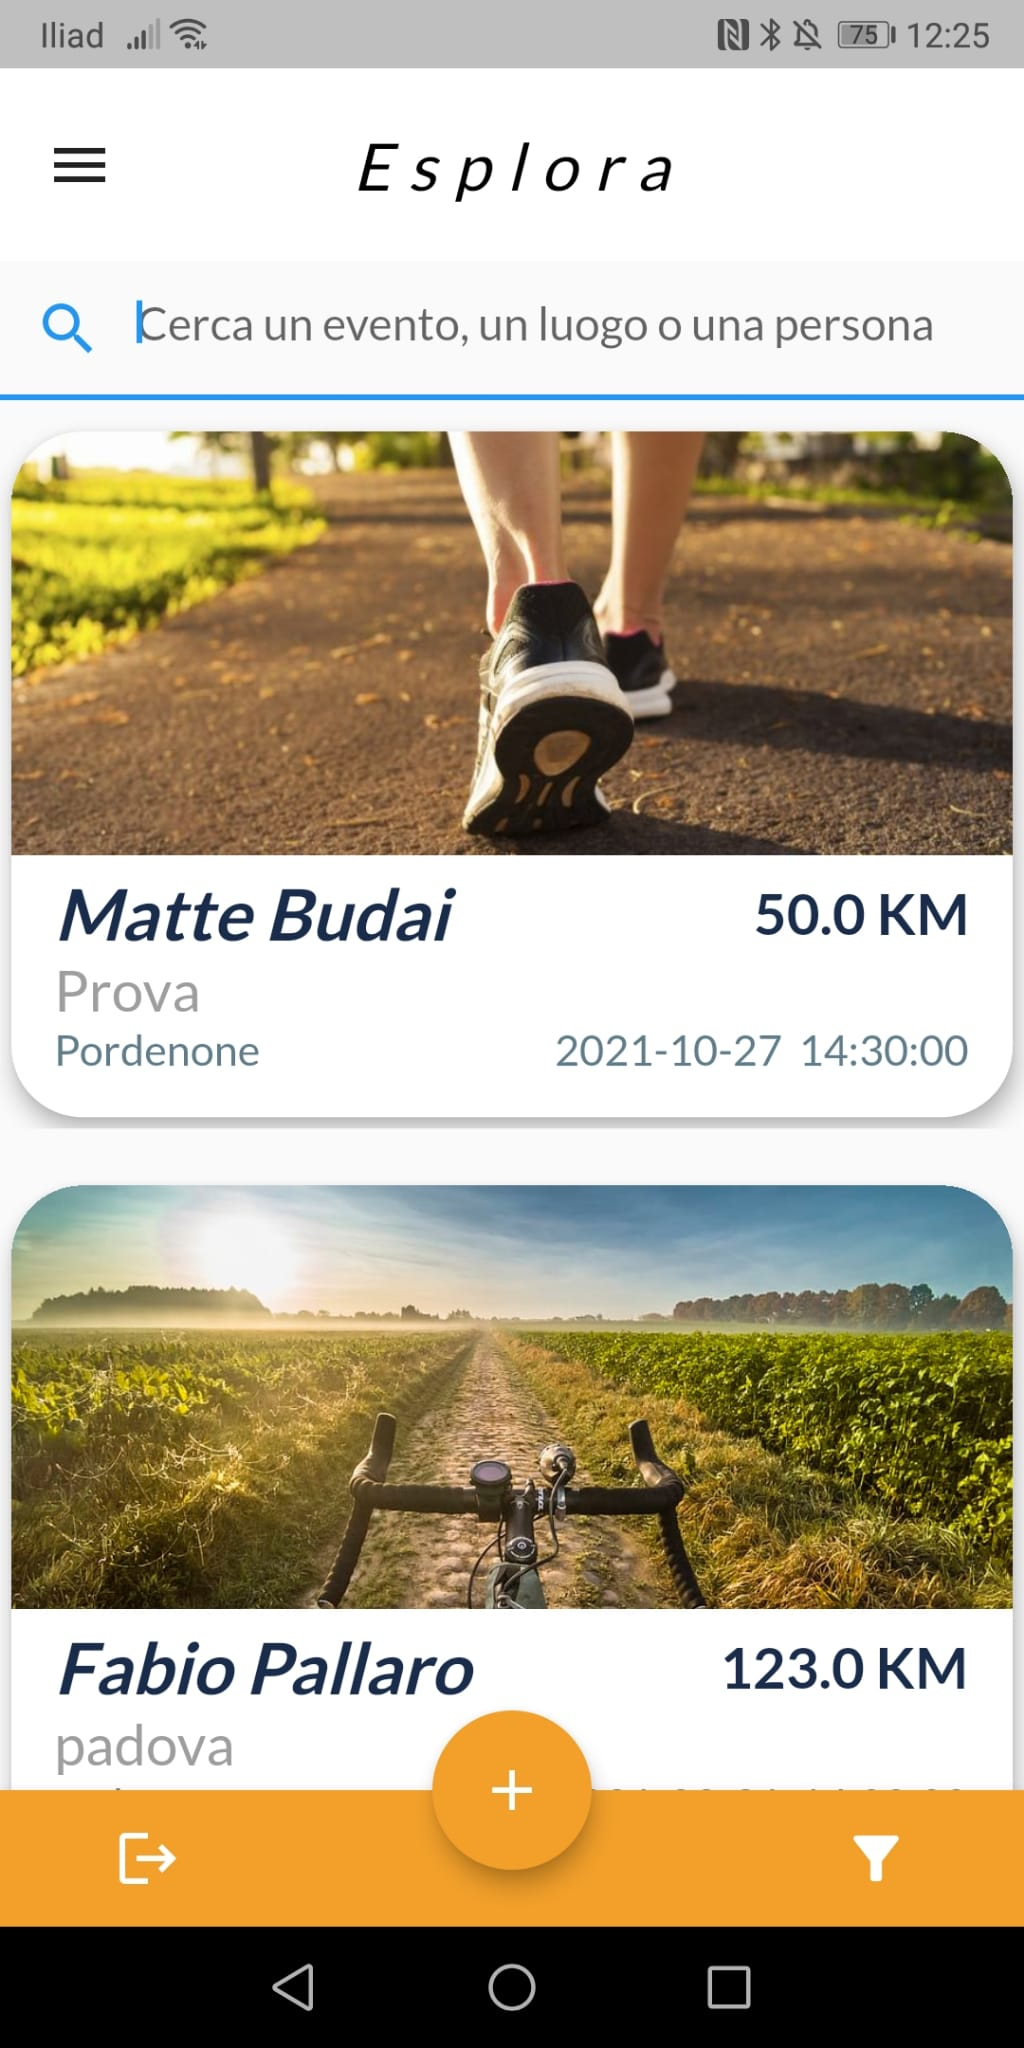
\includegraphics[width=6cm]{immagini/colori.jpeg}
		\caption{Pagina principale}
		\label{fig:Pagina principale}
	\end{minipage}
	\hfill
	\begin{minipage}[b]{0.47\textwidth}
		\centering
		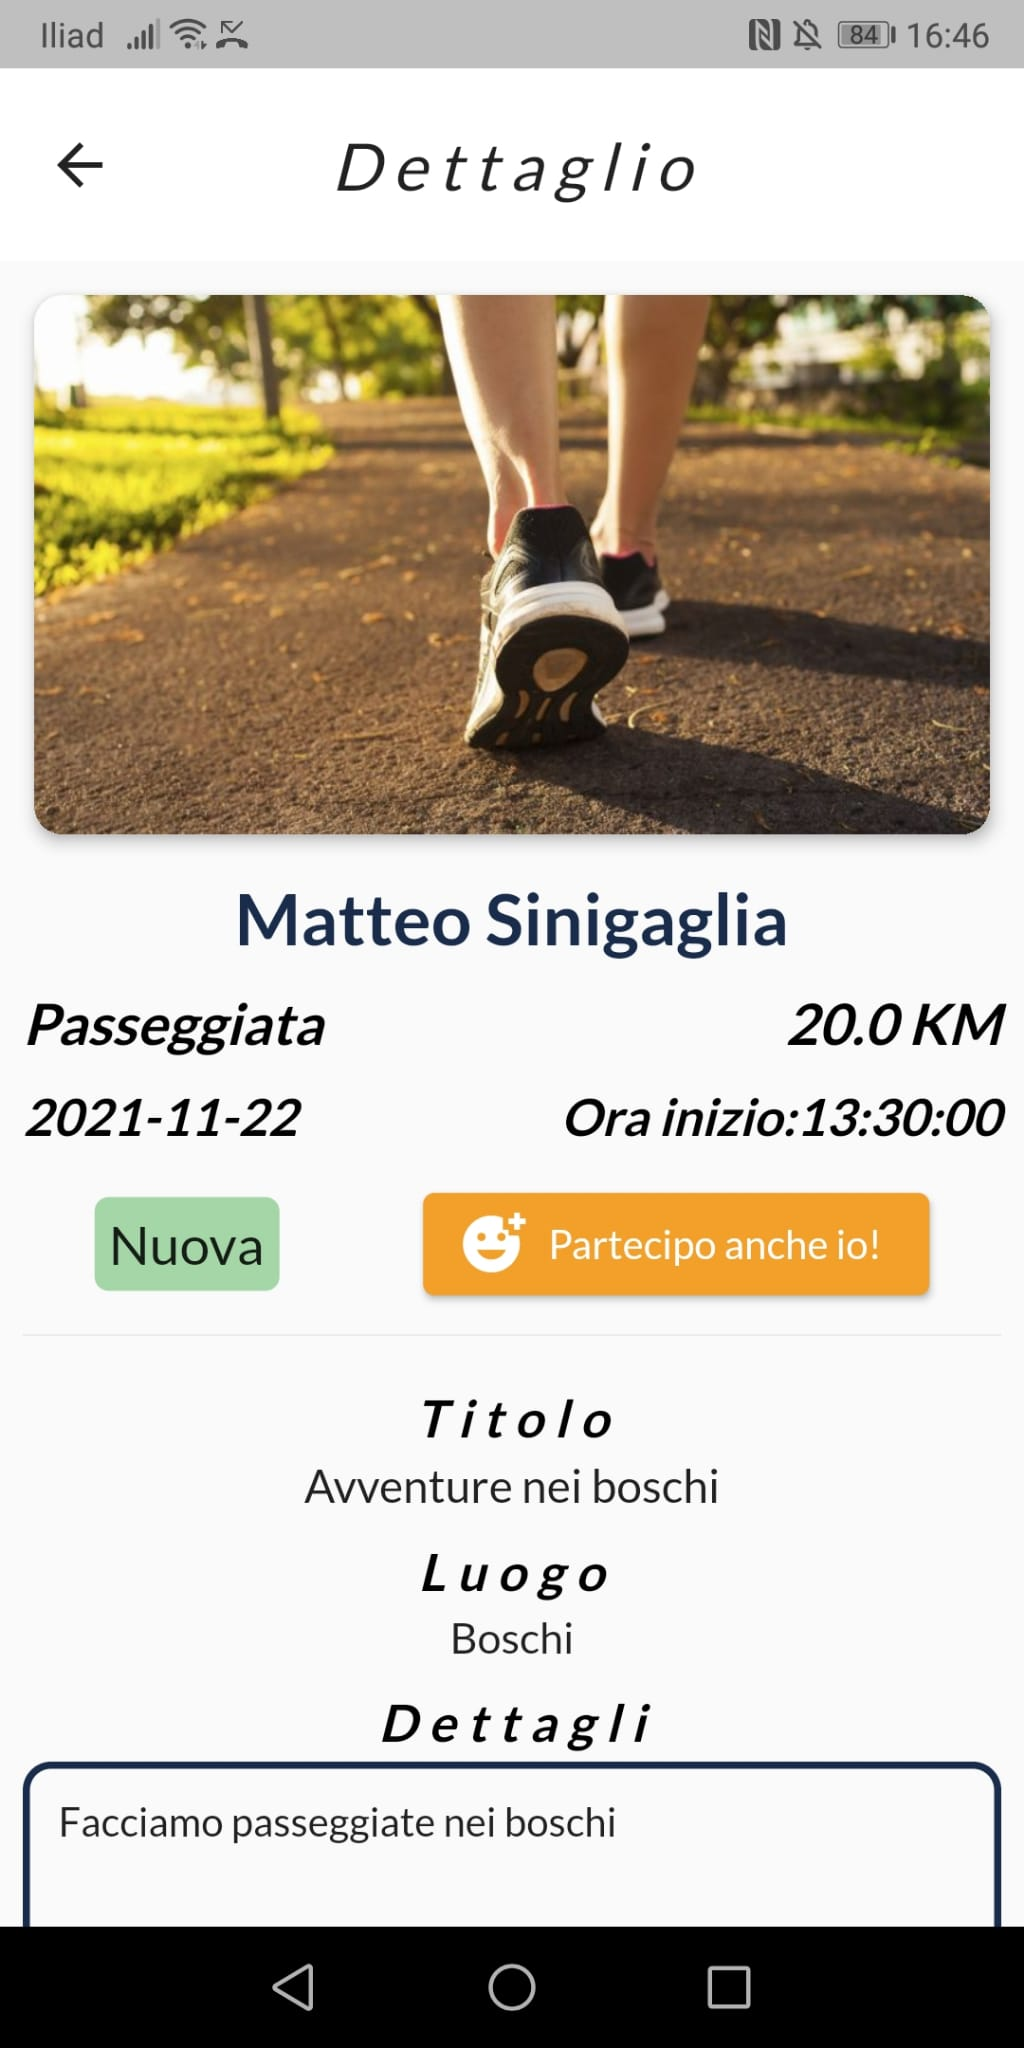
\includegraphics[width=6cm]{immagini/partecipo.jpeg}
		\caption{Schermata di partecipazione}
		\label{fig:Schermata di partecipazione}
	\end{minipage}
\end{figure}
 
 \newpage

\subsection{Organizzazione del progetto}

All'interno del progetto i file sono stati suddivisi nelle varie sottocartelle in base al loro compito.\\
Oltre al file main.dart, che è il file principale dell'applicazione, sono presenti altre 4 cartelle che permettono di organizzare meglio il lavoro:
\begin{itemize}
	\item \textbf{models}: che permette di gestire le eccezioni;
	\item \textbf{providers}: che permette di gestire il modello dei dati e fare le varie chiamate al backend;
	\item \textbf{screens}: che crea tutte le pagine dell'applicazione con gli appositi widget;
	\item \textbf{widgets}: che offrono supporto agli screens tramite la creazione di widget.
\end{itemize}
\begin{figure}[htbp]	
	\centering
	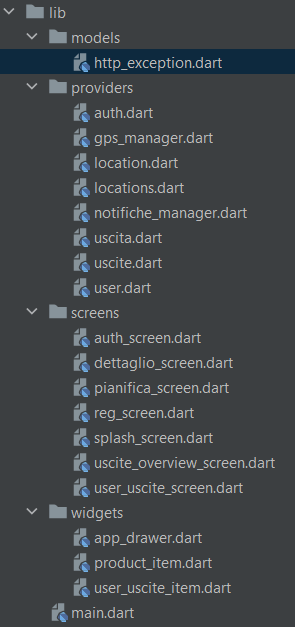
\includegraphics[width=5cm]{immagini/struttura.png}
	\caption{Struttura progetto}
	\label{fig:Struttura progetto}
\end{figure}

\newpage

\section{Tecnologie e strumenti}
Per svolgere il progetto, tralasciando lo studio del framework Flutter e del linguaggio Dart che vengono descritti nel capitolo precedente, è stato necessario utilizzare altri strumenti e tecnologie.\\
Tra questi i principali sono:
\begin{itemize}
	\item Android Studio;
	\item GitLab;
	\item Database DBeaver;
	\item Backend Spring.
\end{itemize}

\subsection{Android Studio}
Android Studio è un IDE per lo sviluppo per la piattaforma Android.\\
Questo IDE, già utilizzato da me in precedenza, è stato configurato correttamente installando i plugin per Flutter e Dart necessari.\\
Android Studio mi ha permesso inoltre di installare e configurare il cellulare così da poter vedere l'applicazione in modo realistico sul mio dispositivo fisico.\\
È molto valido anche perchè fornisce vari dispositivi virtuali su cui testare l'applicazione.

\begin{figure}[htbp]	
	\centering
	
\includegraphics[width=3cm]{immagini/logoandroidstudio.png}
	\caption{Logo Android Studio}
	\label{fig:Logo Android Studio}
\end{figure}

\subsection{GitLab}
GitLab è una piattaforma web open source che permette la gestione di repository Git.\\
Grazie a GitLab è possibile lavorare parallelamente
ad altre persone sullo stesso progetto senza generare conflitti.\\
All'interno della repository presente su GitLab al seguente indirizzo \url{https://gitlab.synclab.it/padovaformazione/sportwill/} viene gestito tutto il progetto ovvero il backend, l'applicazione mobile e la webapp.\\

\begin{figure}[htbp]	
	\centering
	
\includegraphics[width=2cm]{immagini/logogitlab.png}
	\caption{Logo GitLab}
	\label{fig:Logo GitLab}\end{figure}

\newpage

\subsection{Database}
Il database utilizzato per l'applicazione è DBeaver che è gratuito e scaricabile alla seguente pagina \url{https://dbeaver.io/download/}.\\
L'utilizzo del database è stato fondamentale per testare che tutto andasse nella maniera prevista.\\

\begin{figure}[htbp]	
	\centering
	
\includegraphics[width=3cm]{immagini/logodbeaver.png}
	\caption{Logo DBeaver}
	\label{fig:Logo DBeaver}
\end{figure}

\subsection{Backend}
Per gestire i dati sono state fatte delle chiamate al backend.\\
Il backend comprendeva principalmente i linguaggi Spring boot e Spring jpa ed è stato gestito da altri stagisti con il quale sono stato in stretto contatto per organizzare le varie chiamate necessarie, così da definire gli indirizzi e i valori attesi.\\
Tutte queste chiamate erano disponibili su un server gestito dal tutor aziendale Fabio Pallaro.\\

\begin{figure}[htbp]	
	\centering
	
\includegraphics[width=3cm]{immagini/springlogo.png}
	\caption{Logo Spring}
	\label{fig:Logo Spring}
\end{figure}

\newpage

\section{Analisi dei requisiti}
In questa sezione viene descritta l'analisi dei requisti con i  vari casi d'uso individuati e successivamente viene effettuato il tracciamento.

\subsection{Casi d'uso}
In un primo momento, per determinare i casi d'uso, sono stati definiti gli attori principali dell'applicazione.
Tra questi sono state identificate tre tipologie:
\begin{itemize}
	\item Utente non autenticato;
	\item Utente autenticato;
	\item Utente ospite.
\end{itemize}
Successivamente sono stati definiti i quattro casi d'uso principali:
\begin{itemize}
	\item Visualizzazione mappa;
	\item Visualizzazione mappa a schermo intero;
	\item Filtro base;
	\item Filtro avanzato.
\end{itemize}


\subsubsection{ UC1 - Visualizzazione mappa}

	\textbf{Attori Primari:} Utente autenticato e utente ospite.\\
	\textbf{Descrizione:} L'utente vuole vedere la mappa dell'attività selezionata.\\
	\textbf{Scenario principale:} L'utente si trova nella schermata principale dell'applicazione e preme sulla card dell'attività a cui è interessato. Se questa attività è iniziata e contiene dati relativi alla posizione verrà mostrata la mappa altrimenti non comparirà tra i dettagli.\\
	\textbf{Precondizione:} L'utente si trova nella schermata principale dell'applicazione e preme su una card.\\
	\textbf{Postcondizione:} Se l'attività selezionata conterrà dati relativi alla posizione verrà mostrata una mappa con punto di partenza, percorso svolto e punto attuale o finale.\\


\subsubsection{ UC2 - Visualizzazione mappa a schermo intero}

\textbf{Attori Primari:} Utente autenticato e utente ospite.\\
\textbf{Descrizione:} L'utente vuole vedere la mappa a schermo intero per navigare meglio.\\
\textbf{Scenario principale:} L'utente sta visualizzando le specifiche di un'attività e tra queste è presente pure la mappa, per poterla usare più comodamente deve premere sul bottone che la ingrandisce a schermo intero.\\
\textbf{Precondizione:} L'utente si trova nelle specifiche di un'attività e tra i dettagli è presente anche la mappa. Una volta individuata preme sul bottone per renderla a schermo intero.\\
\textbf{Postcondizione:} La mappa viene visualizzata a schermo intero così da facilitarne l'utilizzo.\\

\subsubsection{ UC3 - Filtro base}

\textbf{Attori Primari:} Utente autenticato e utente ospite.\\
\textbf{Descrizione:} L'utente cerca un'attività in base al luogo, al titolo e alla persona che ha creato l'attività digitando su una casella di ricerca.\\
\textbf{Scenario principale:} L'utente si trova nella pagina principale dell'applicazione e vuole cercare l'attività effettuata da un altro utente. Per cercarla basterà che inizierà a digitare il nome o il cognome della persona desiderata e compariranno solo le card che contengono quanto appena scritto.\\
\textbf{Precondizione:} L'utente si trova nella pagina principale dell'applicazione e inizia a scrivere nella casella di ricerca.\\
\textbf{Postcondizione:} Vengono visualizzate solo le card che contengono nel titolo, nel nome, nel cognome o nel luogo quello scritto dall'utente.\\

\subsubsection{ UC4 - Filtro avanzato}

\textbf{Attori Primari:} Utente autenticato e utente ospite.\\
\textbf{Descrizione:} L'utente si trova nella pagina principale dell'applicazione e aprendo il menù dei filtri può applicarli in base alle sue esigenze.\\
\textbf{Scenario principale:} L'utente apre il menù dei filtri e seleziona la data di inizio o lo sport che gli interessano e preme sull'icona del check per applicarli così da vedere solo le card con quella tipologia di sport e a partire da quella data.\\
\textbf{Precondizione:} L'utente si trova nel menù dei filtri, riempe alcuni campi e preme sull'icona del check.\\
\textbf{Postcondizione:} L'utente visualizza solo le card che rispettano i valori messi nel filtro in precedenza. Per aiutare l'utente e far capire che il filtro è stato applicato, l'icona che porta al menù dei filtri cambia colore in verde.\\

\newpage

\subsection{Tracciamento requisti}
I requisiti individuati sono tutti fondamentali e obbligatori e possono essere:
\begin{itemize}
	\item \textbf{Funzionali}: legati alle funzionalità offerte dal sistema;
	\item \textbf{Qualitativi}: rappresentanti standard e metriche da seguire per garantire la qualità del sistema;
	\item \textbf{Di Vincolo}: dipendenti da fattori esterni o di dominio.
\end{itemize}
Per ogni requisito delle tabelle sottostanti è stata decisa la seguente struttura: 
\begin{itemize}
	\item\textbf{Requisito:} R[Tipologia][Identificativo];
	\item\textbf{Descrizione:} descrizione breve ma completa del requisito, meno ambigua possibile;
	\item\textbf{Fonti:} ogni requisito può derivare dalle seguenti fonti:
	\begin{itemize}
		\item Azienda: si tratta di un requisito individuato con l'azienda;
		\item Caso d'uso: si tratta di un requisito estrapolato dai casi d'uso individuati.
	\end{itemize}
\end{itemize}

\subsubsection{Requisiti funzionali}

\begin{center}
	\begin{table}[h!]
		
		\label{tab:Requisiti funzionali}
		\begin{tabularx}{\textwidth}{|c|p{8cm}|p{2.1cm}|}
			
			\hline
			\textbf{Requisito} & \centering\textbf{Descrizione} & \textbf{Fonti}  \\\hline
			
			RF1 & Se per un'attività ci sono coordinate relative alla posizione deve essere possibile visualizzare la mappa  & UC1\\
			\hline	
			RF2 &Se presente la mappa, la stessa deve essere possibile da visualizzare a schermo intero. & UC2\\
			\hline
			RF3& Deve essere possibile cercare le attività per titolo, luogo, nome e cognome.	& UC3	\\
			\hline	
			RF4& Deve essere possibile applicare i filtri avanzati. Tra questi bisogna poter filtrare in base al tipo di sport, la data di inizio, di fine e se si riferiscono ad attività create da me.	& UC4	\\
			\hline		
		\end{tabularx}
		\vspace{0.3cm}
		\caption{Requisiti funzionali}
	\end{table}
\end{center}

\newpage

\subsubsection{Requisiti qualitativi}

\begin{center}
	\begin{table}[h!]
		
		\label{tab:Requisiti qualitativi}
		\begin{tabularx}{\textwidth}{|c|p{8cm}|p{2.1cm}|}
			
			\hline
			\textbf{Requisito} & \centering\textbf{Descrizione} & \textbf{Fonti}  \\\hline
			
			RQ1 &Il codice scritto dovrà essere versionabile tramite Git.  & Azienda\\
			\hline	
			RQ2 &Il repository utilizzato sarà quello presente su GitLab. & Azienda\\
			\hline
			RQ3& Per implementare le funzionalità bisognerà usare il framework Flutter con linguaggio Dart.	& Azienda	\\
			\hline		
		\end{tabularx}
		\vspace{0.3cm}
		\caption{Requisiti qualitativi}
	\end{table}
\end{center}

\subsubsection{Requisiti di vincolo}

\begin{center}
	\begin{table}[h!]
		
		\label{tab:Requisiti di vincolo}
		\begin{tabularx}{\textwidth}{|c|p{8cm}|p{2.1cm}|}
			
			\hline
			\textbf{Requisito} & \centering\textbf{Descrizione} & \textbf{Fonti}  \\\hline
			
				RV1 & Tutti i dati dovranno essere memorizzati nel back-end.  & Azienda\\
				\hline
				RV2 & Per le chiamate verrà utilizzato un server fornito dall'azienda.  & Azienda\\
			\hline		
		\end{tabularx}
		\vspace{0.3cm}
		\caption{Requisiti di vincolo}
	\end{table}
\end{center}


\newpage

\section{Implementazioni}
Oltre al completamento dei requisiti sono state effettuate altre implementazioni.\\
Nel complesso le funzionalità realizzate durante lo stage sono state: 
\begin{itemize}
	\item Logo;
	\item Filtro di ricerca testo;
	\item Pagina Modifica e campi obbligatori;
	\item Mappa percorso;
	\item Aggiornamento automatico mappa;
	\item Mappa schermo intero;
	\item Colori;
	\item Pagina Modifica;
	\item Eliminazione, Modifica e Aggiunta di un'attività;
	\item Filtro avanzato di ricerca attività;
	\item Pubblicazione applicazione Play Store.
\end{itemize}
Tutti i servizi sono stati rilasciati su un'apposita repository aziendale su \textit{GitLab}.

\subsection{Logo}
È stato modificato il logo di base di Flutter con quello di Sportwill.\\
Per  fare ciò è stato inserita l'immagine del logo all'interno della seguente cartella \textit{app/src/main/res/mipmap/}.\\
In alternativa si poteva definire nel file \textit{pubspec.yaml} il percorso del logo dell'applicazione e poi inserire l'immagine del logo nella cartella appena definita.\\

\begin{figure}[htbp]	
	\centering
	
\includegraphics[width=6cm]{immagini/logosportwill.png}
	\caption{Logo Sportwill}
	\label{fig:Logo Sportwill}
\end{figure}

\newpage

\subsection{Filtro di ricerca testo}
All'interno della pagina principale dell'applicazione ovvero la pagina \textit{uscite\_overview\_screen.dart} è stato aggiunto un widget che permette di ricercare le varie card in base all'evento, al luogo o alla persona.\\
Digitando nella barra di ricerca si potranno ricercare solo le card a cui si è interessati.\\
Per fare ciò è stato inserita una funzione chiamata \textit{ricerca()} che ritorna una TextField come Widget sempre nel file \textit{uscite\_overview\_screen.dart}.\\

\begin{figure}[htbp]	
	\centering
	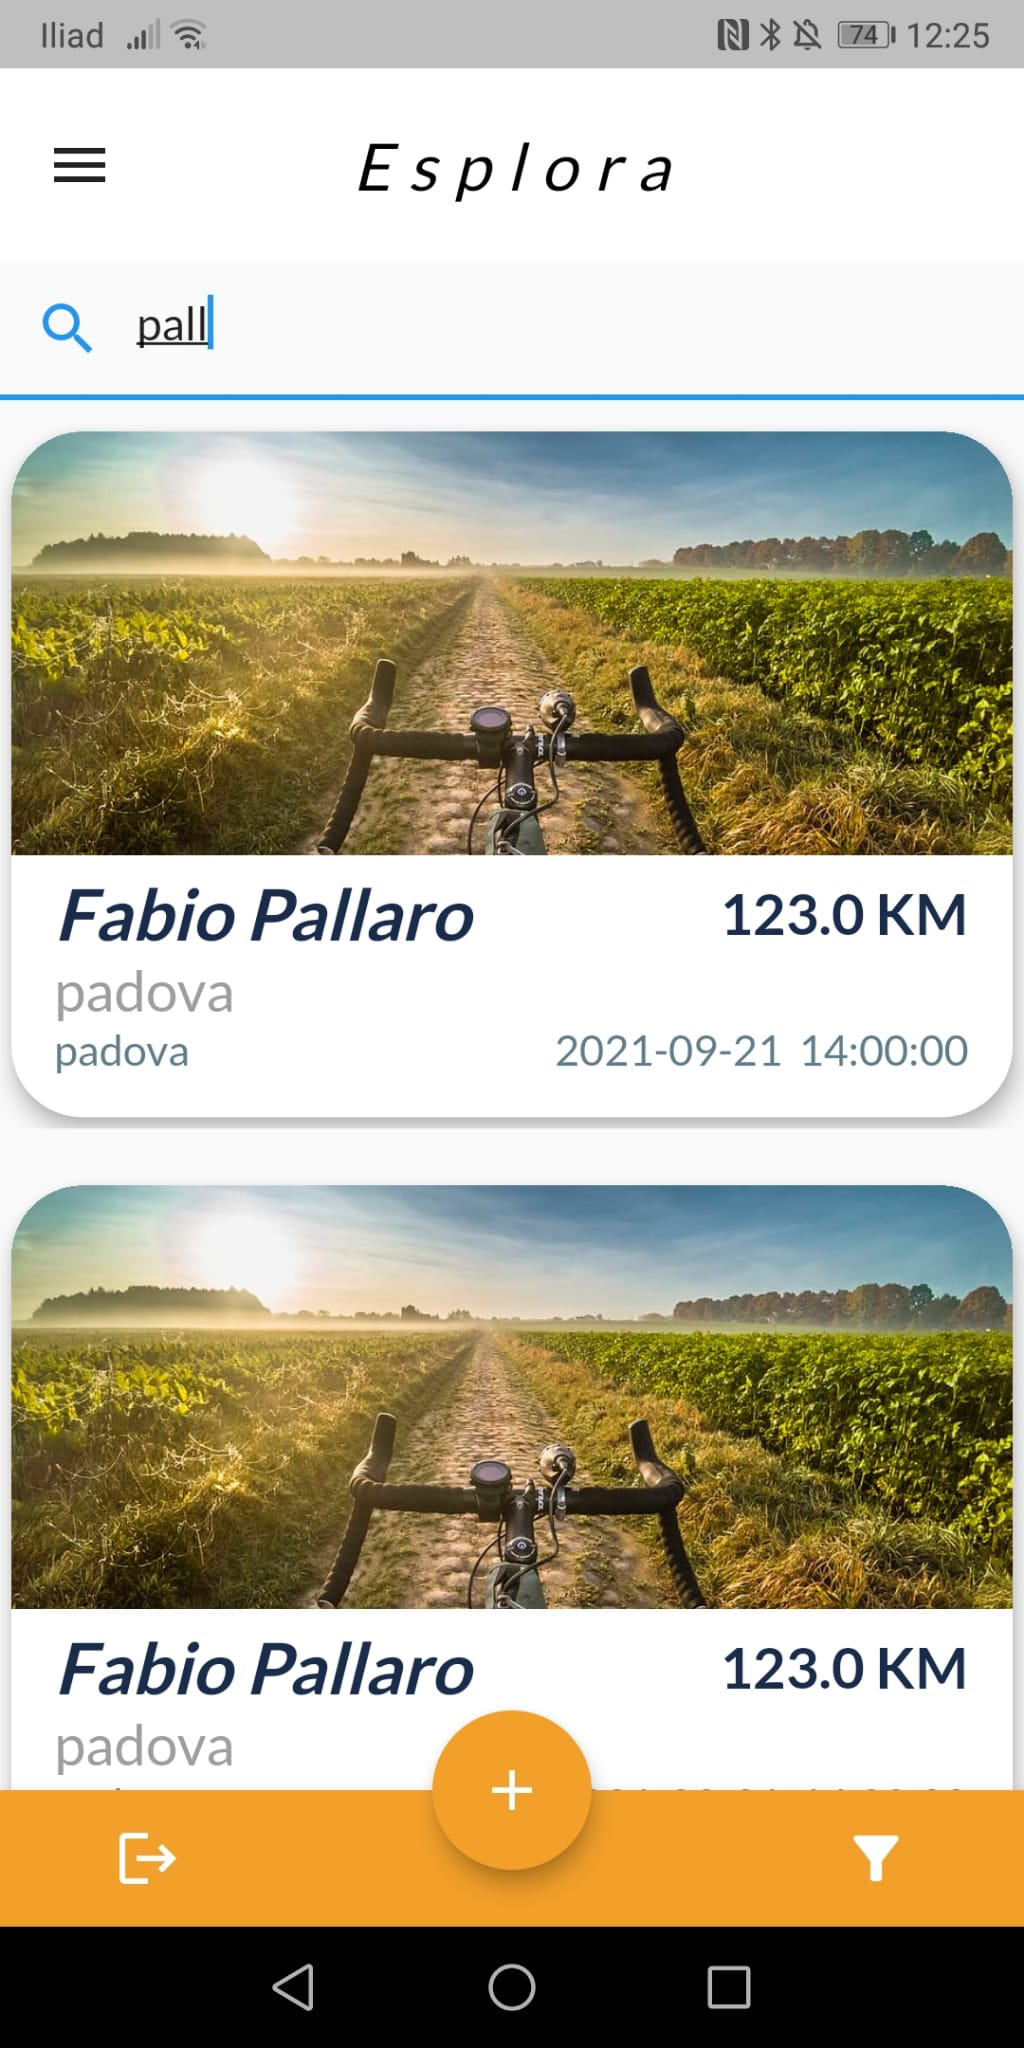
\includegraphics[width=6cm]{immagini/filtrotesto.jpeg}
	\caption{Filtro di ricerca testo}
	\label{fig:Filtro di ricerca testo}
\end{figure}

\newpage

\subsection{Campi obbligatori e pagina modifica e crea}
All'interno di questa pagina sono stati tolti tutti i campi obbligatori non richiesti.\\
Per fare ciò sono stati eliminati tutti i validator non necessari nel file \textit{pianifica\_screen.dart} e lasciato i restanti con le apposite funzioni.\\
Inoltre all'interno di questa pagina sono stati aggiustati i campi degli orari in quanto nella funzione \textit{selezionaOra()} tornava i minuti attuali.\\
Per rendere all'utente più comprensibile il salvataggio è stata sostituita l'icona precedente di salvataggio con l'icona \textit{Icon(Icons.save)}.\\

\begin{figure}[htbp]	
	\centering
	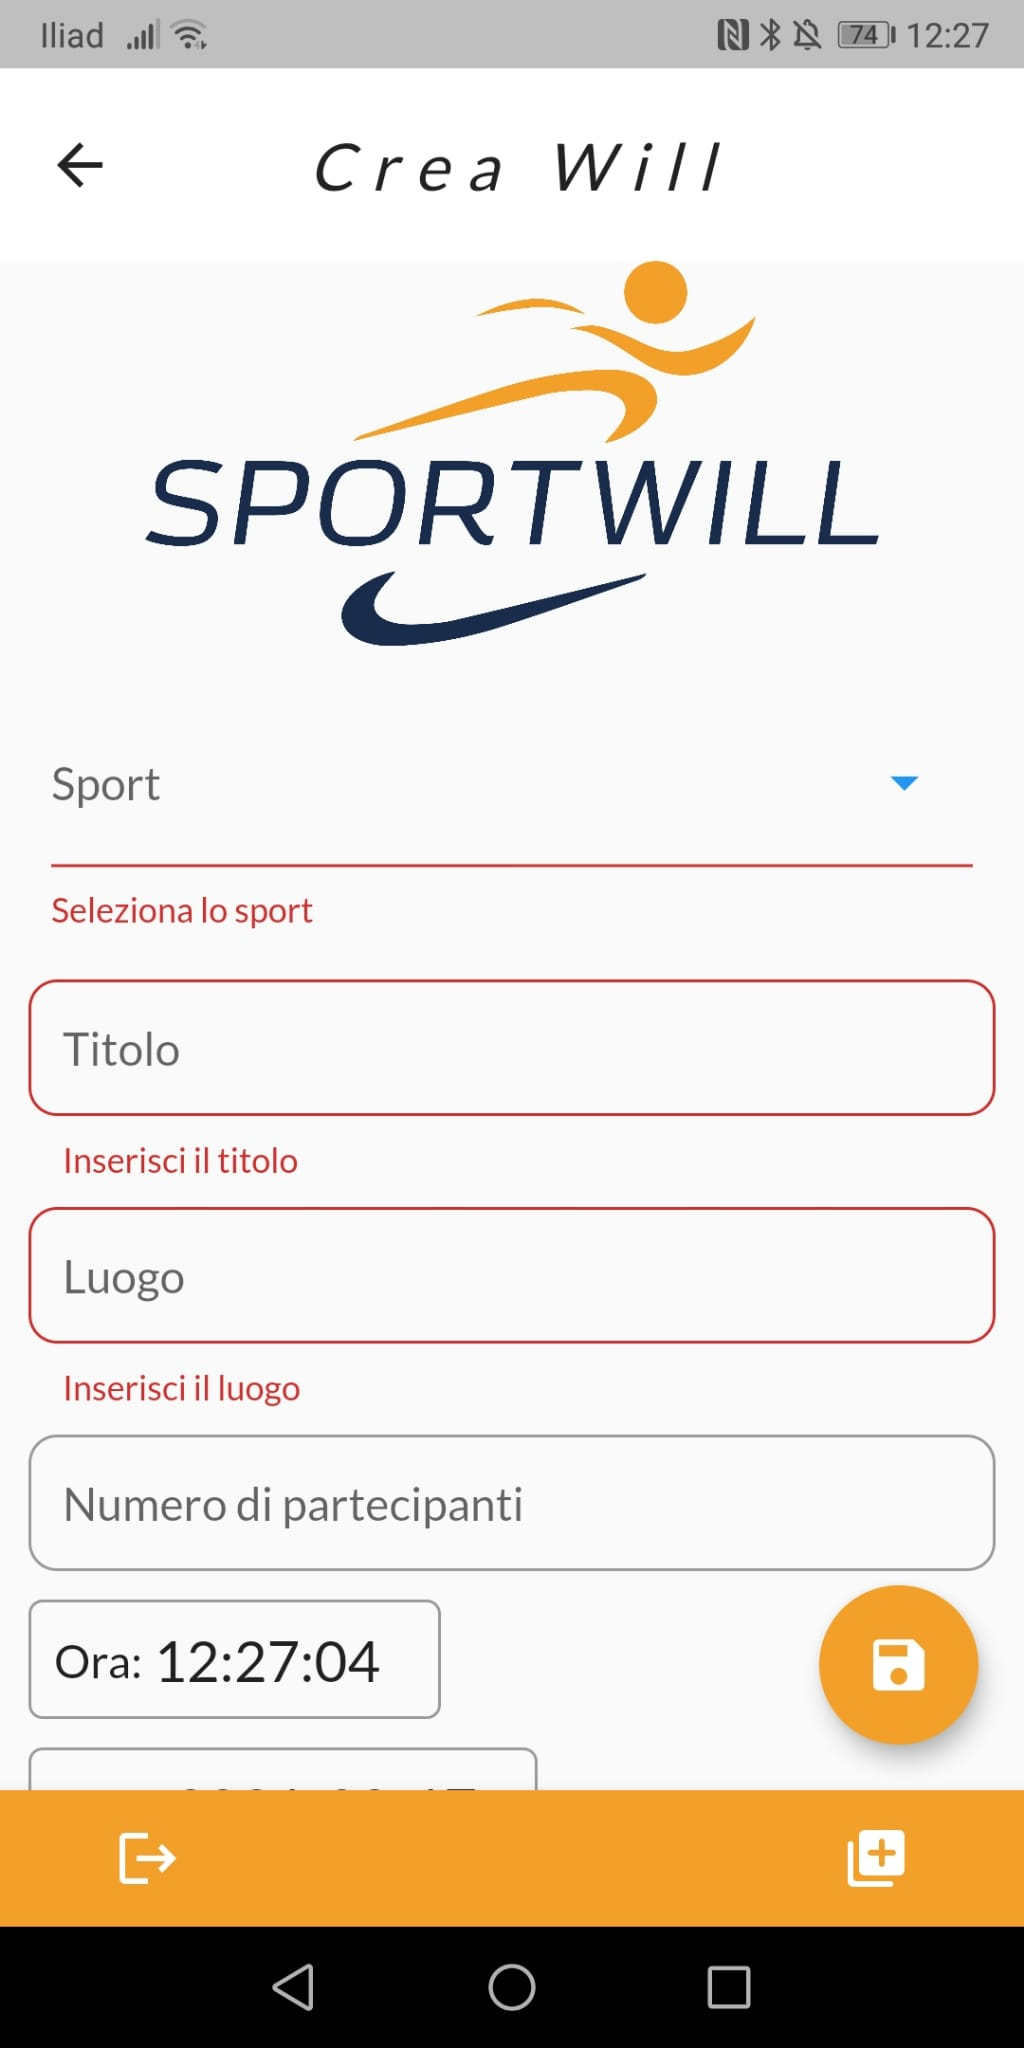
\includegraphics[width=6cm]{immagini/modifica.jpeg}
	\caption{Campi obbligatori}
	\label{fig:Campi obbligatori}
\end{figure}

\newpage

\subsection{Colori}
All'interno dei vari file, sono stati cambiati diversi colori, in modo che venissero utilizzati principalmente quelli definiti nell'applicazione, ovvero il bianco e l'arancione.\\

\begin{figure}[htbp]	
	\centering
	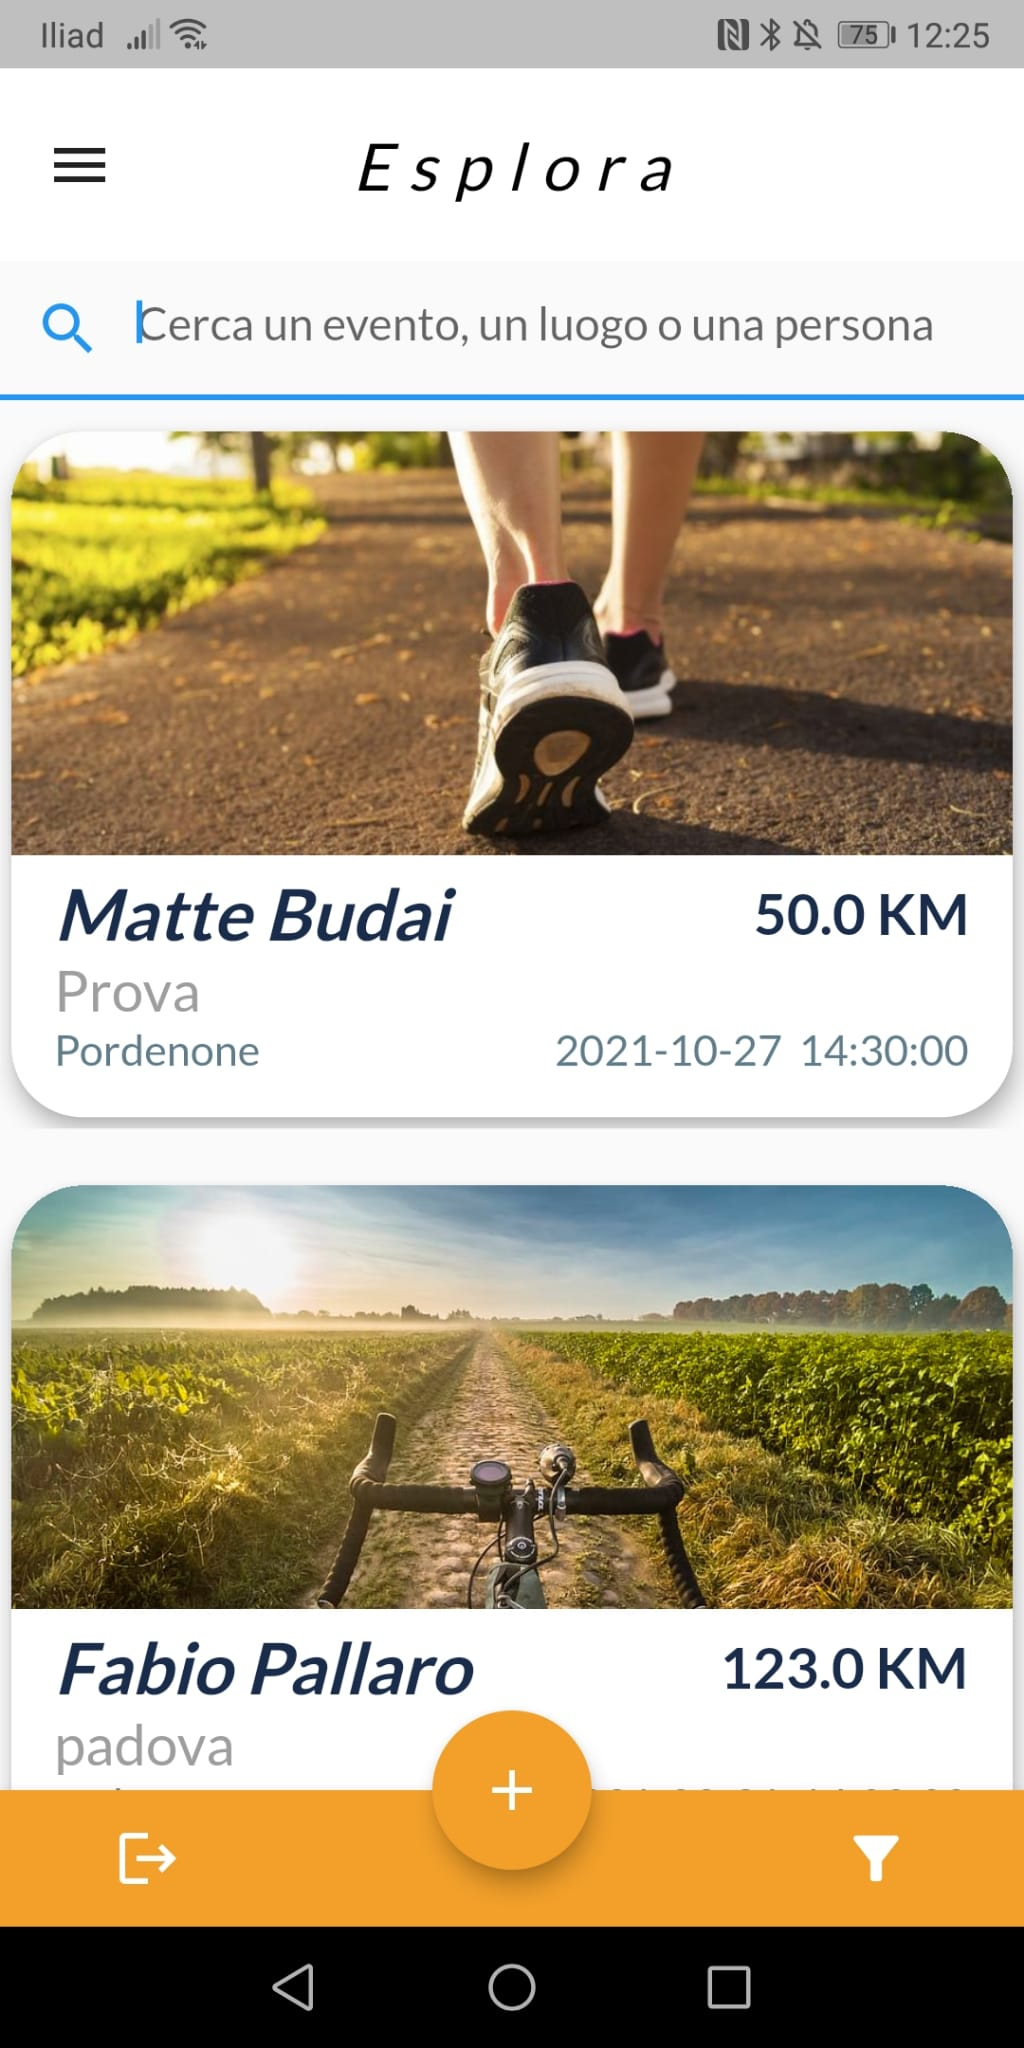
\includegraphics[width=6cm]{immagini/colori.jpeg}
	\caption{Colori}
	\label{fig:Colori}
\end{figure}


\subsection{Eliminazione, Modifica e Aggiunta di un'attività}
In seguito alle modifiche di vari campi, sono state sistemate le pagine di eliminazione, modifica e aggiunta di un'attività con nuovi valori e formati in modo che venissero rispettate le richieste del backend.\\
In particolar modo sono stati sistemati i valori che riguardavano la data e l'orario con i nuovi formati richiesti. Inoltre la lunghezza e il numero di partecipanti richiedevano rispettivamente un double e un intero.

\newpage

\subsection{Mappa percorso}
Per gestire la mappa sono stati creati due providers:
\begin{itemize}
	\item location.dart: che è il modello e contiene tutti i dati che riguardano una posizione;
	\item locations.dart: che permette di chiamare il backend per ottenere i vari valori da visualizzare nella mappa.
\end{itemize}
La mappa viene creata nel file \textit{dettaglio\_screen.dart} e viene mostrata solo se c'è almeno una posizione nel database per l'attività selezionata.\\
Per visualizzare la mappa viene usato Leaflet, una libreria JavaScript per sviluppare mappe geografiche interattive, e viene creato un array a cui vengono aggiunte con una chiamata tutte le posizioni relative a quell'attività.\\ 
Queste posizioni vengono poi disegnate sulla mappa mettendo un marker di colore arancione sulla prima posizione e successivamente vengono collegate in ordine temporale tutte le altre posizioni presenti nell'array con una riga viola fino ad arrivare all'ultima che avrà un marker di colore verde.\\

\begin{figure}[htbp]	
	\centering
	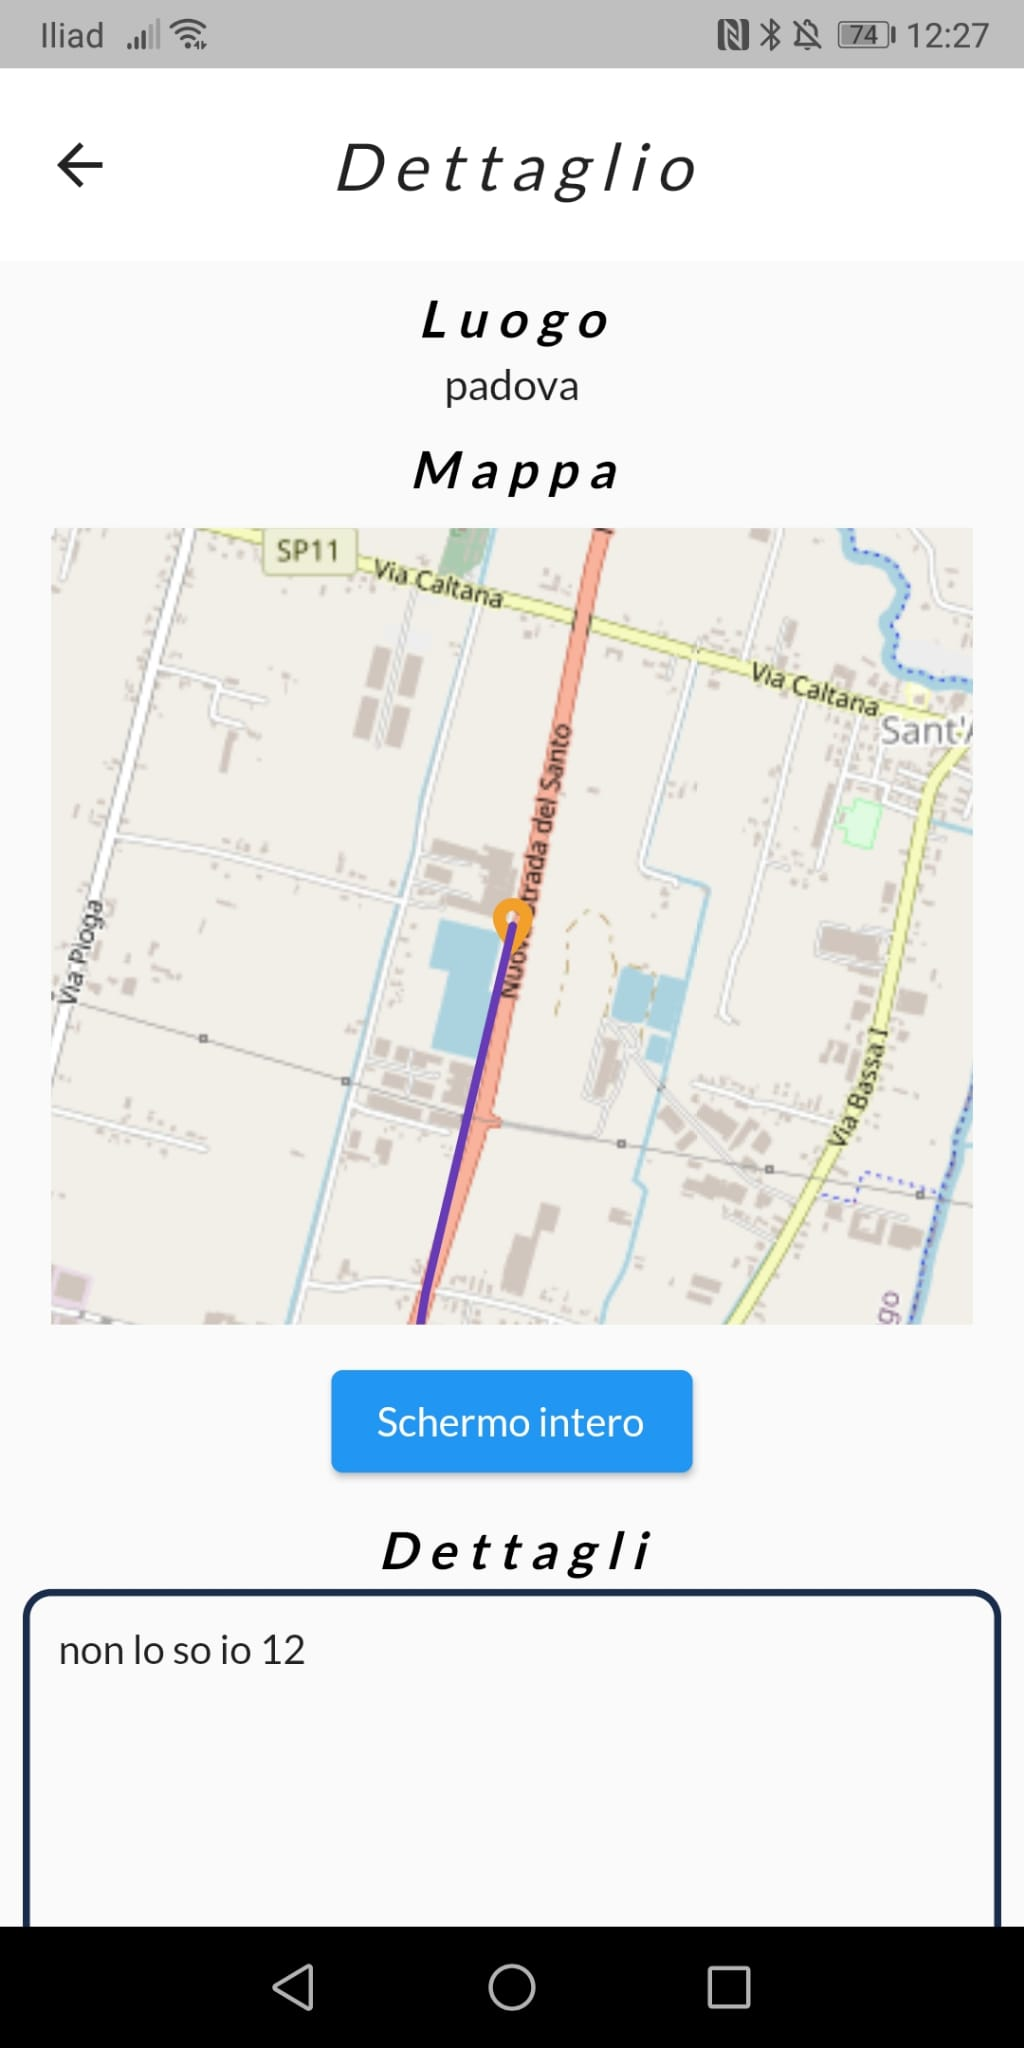
\includegraphics[width=6cm]{immagini/mappa.jpeg}
	\caption{Mappa percorso}
	\label{fig:Mappa percorso}
\end{figure}

\newpage

\subsection{Aggiornamento automatico mappa}
Per fare in modo che la mappa si aggiorni in modo automatico è stato inserito un Timer che ogni 30 secondi va a chiamare la funzione che ritorna tutte le posizioni di quell'attività, così da aggiornare l'array descritto precedentemente.\\
Per evitare che il Timer sia ricostruito ogni volta è stato usato un valore booleano che permette la costruzione del Timer solo la prima volta.\\

\begin{figure}[htbp]	
	\centering
	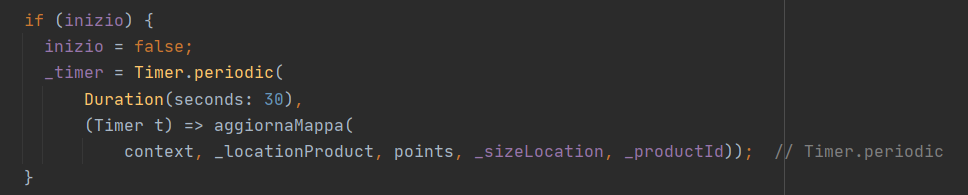
\includegraphics[width=14cm]{immagini/automatico.png}
	\caption{Aggiornamento automatico mappa}
	\label{fig:Aggiornamento automatico mappa}
\end{figure}

\newpage

\subsection{Mappa schermo intero}
Per fare in modo che la mappa sia più utilizzabile e scorrevole all'utente è stata creata la possibilità di vederla a schermo intero.\\
Per fare ciò è stato usato un valore booleano, ovvero \textit{ingradisci}, inizialmente uguale a false, che se impostato uguale a true permetteva di vedere nello schermo solo la mappa.\\
Cliccando sul bottone \textit{schermo intero} viene infatti settato questo valore a true e istantaneamente viene ricostruita la pagina con la mappa a schermo intero.\\
Una volta che la mappa è a schermo intero, premendo sull'icona con la croce in alto a destra viene settato il booleano a false, ricostruendo la pagina come in precedenza con tutti i dettagli dell'attività.\\

\begin{figure}[htbp]	
	\centering
	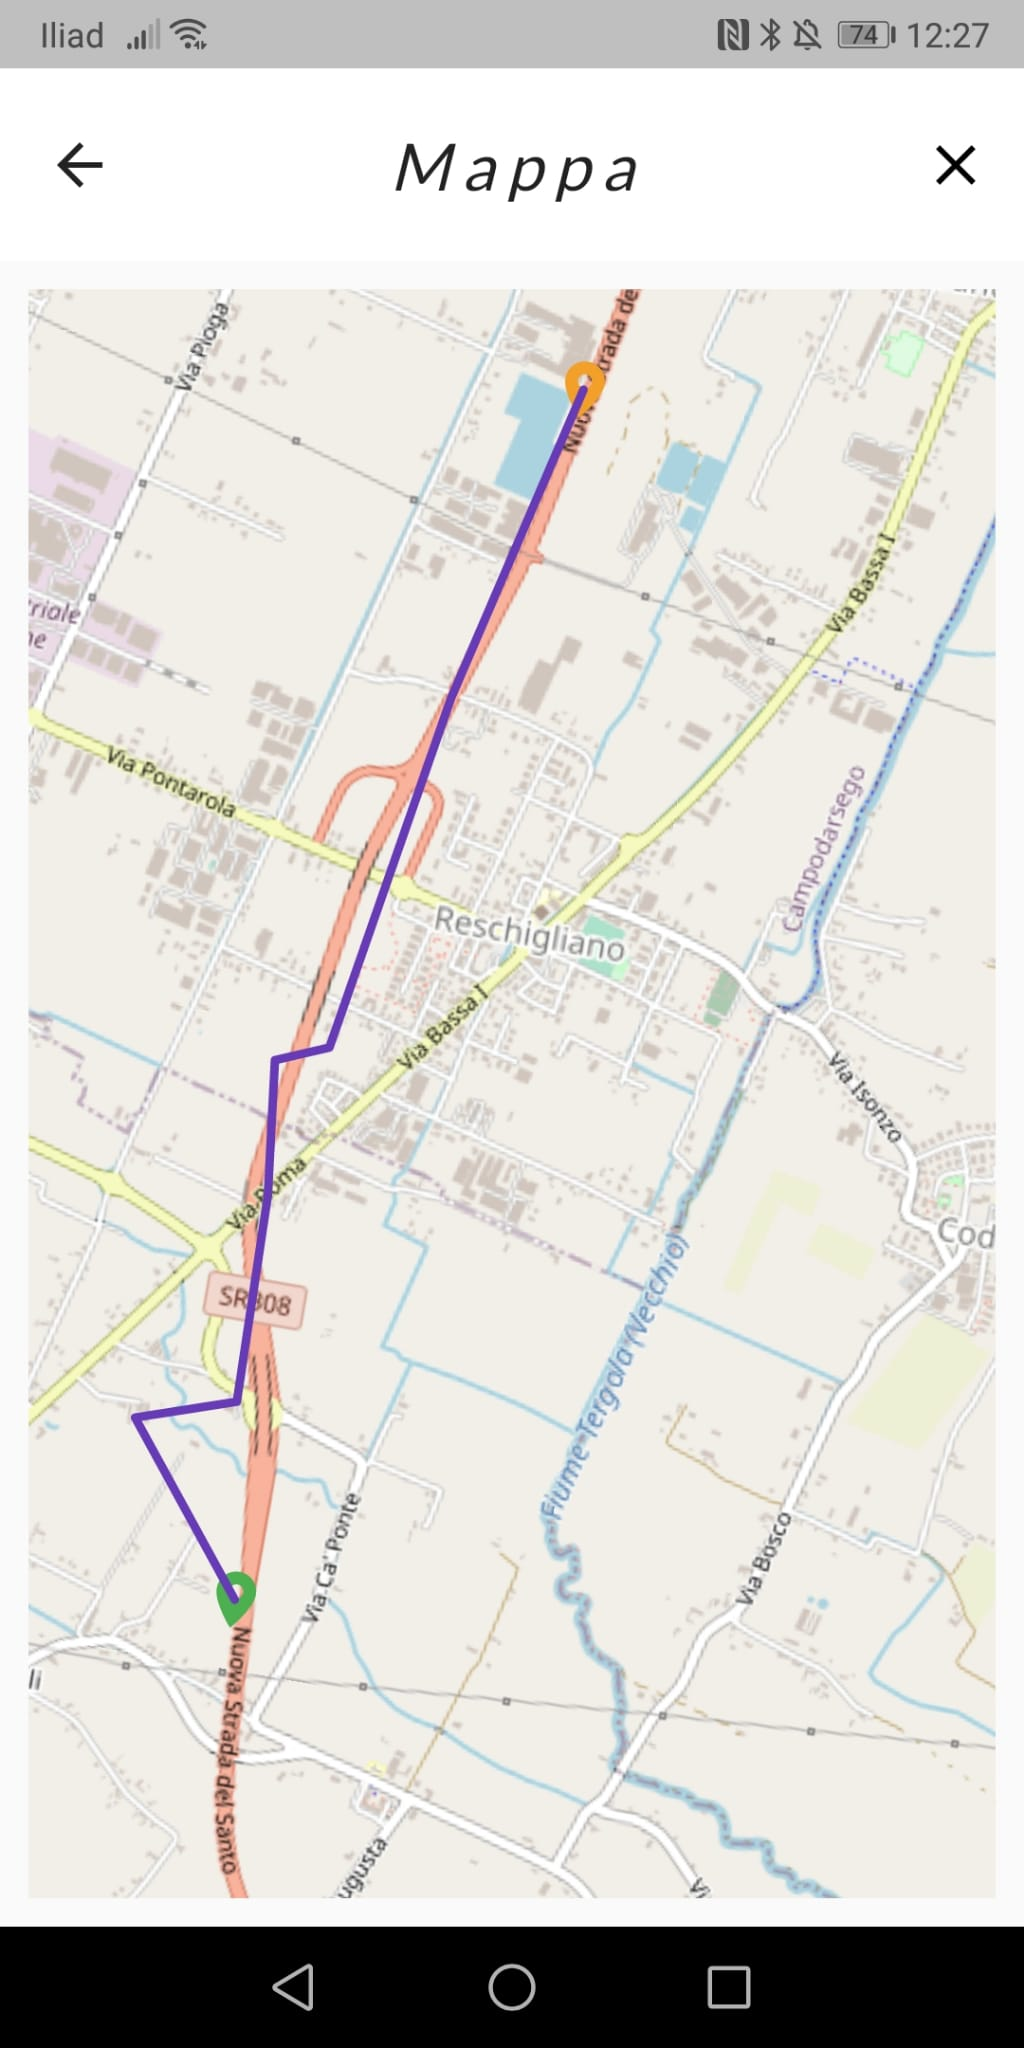
\includegraphics[width=6cm]{immagini/mappaintero.jpeg}
	\caption{Mappa schermo intero}
	\label{fig:Mappa schermo intero}
\end{figure}

\newpage

\subsection{Filtro avanzato di ricerca attività}
Per creare il filtro avanzato è stata creata una funzione \textit{showFilterMenu()} nel file \textit{uscite\_overview\_screen.dart} che contiene una \textit{showDialog}.\\
Per aprire il menù dei filtri bisognerà premere sull'icona dei filtri situata in basso a destra.\\
All'interno di questo menu è possibile filtrare le attività in base allo sport, alla data e se si tratta di tue attività.\\
Per applicare i vari filtri basterà premere sull'icona check.
Una volta premuto sull'icona, viene ricostruita la pagina e impostato il valore booleano che gestisce il filtro uguale a true.\\
Subito dopo aver letto il valore uguale a true, va chiamare nel provider \textit{uscite.dart} la funzione \textit{findBySporteData} che ritorna solo le card che rispettano i valori messi nel filtro.\\
L'icona con la croce, una volta premuta, setta il valore del filtro a false e ricostruisce la pagina chiudendo la showdialog(menù) dei filtri e cancellando i filtri precedentemente applicati.\\
Per poter capire se abbiamo applicato i filtri basterà guardare se l'icona dei filtri ha il colore verde.
Invece se non avremo filtri applicati l'icona avrà il solito colore bianco.

\begin{figure}[htbp]	
	\centering
	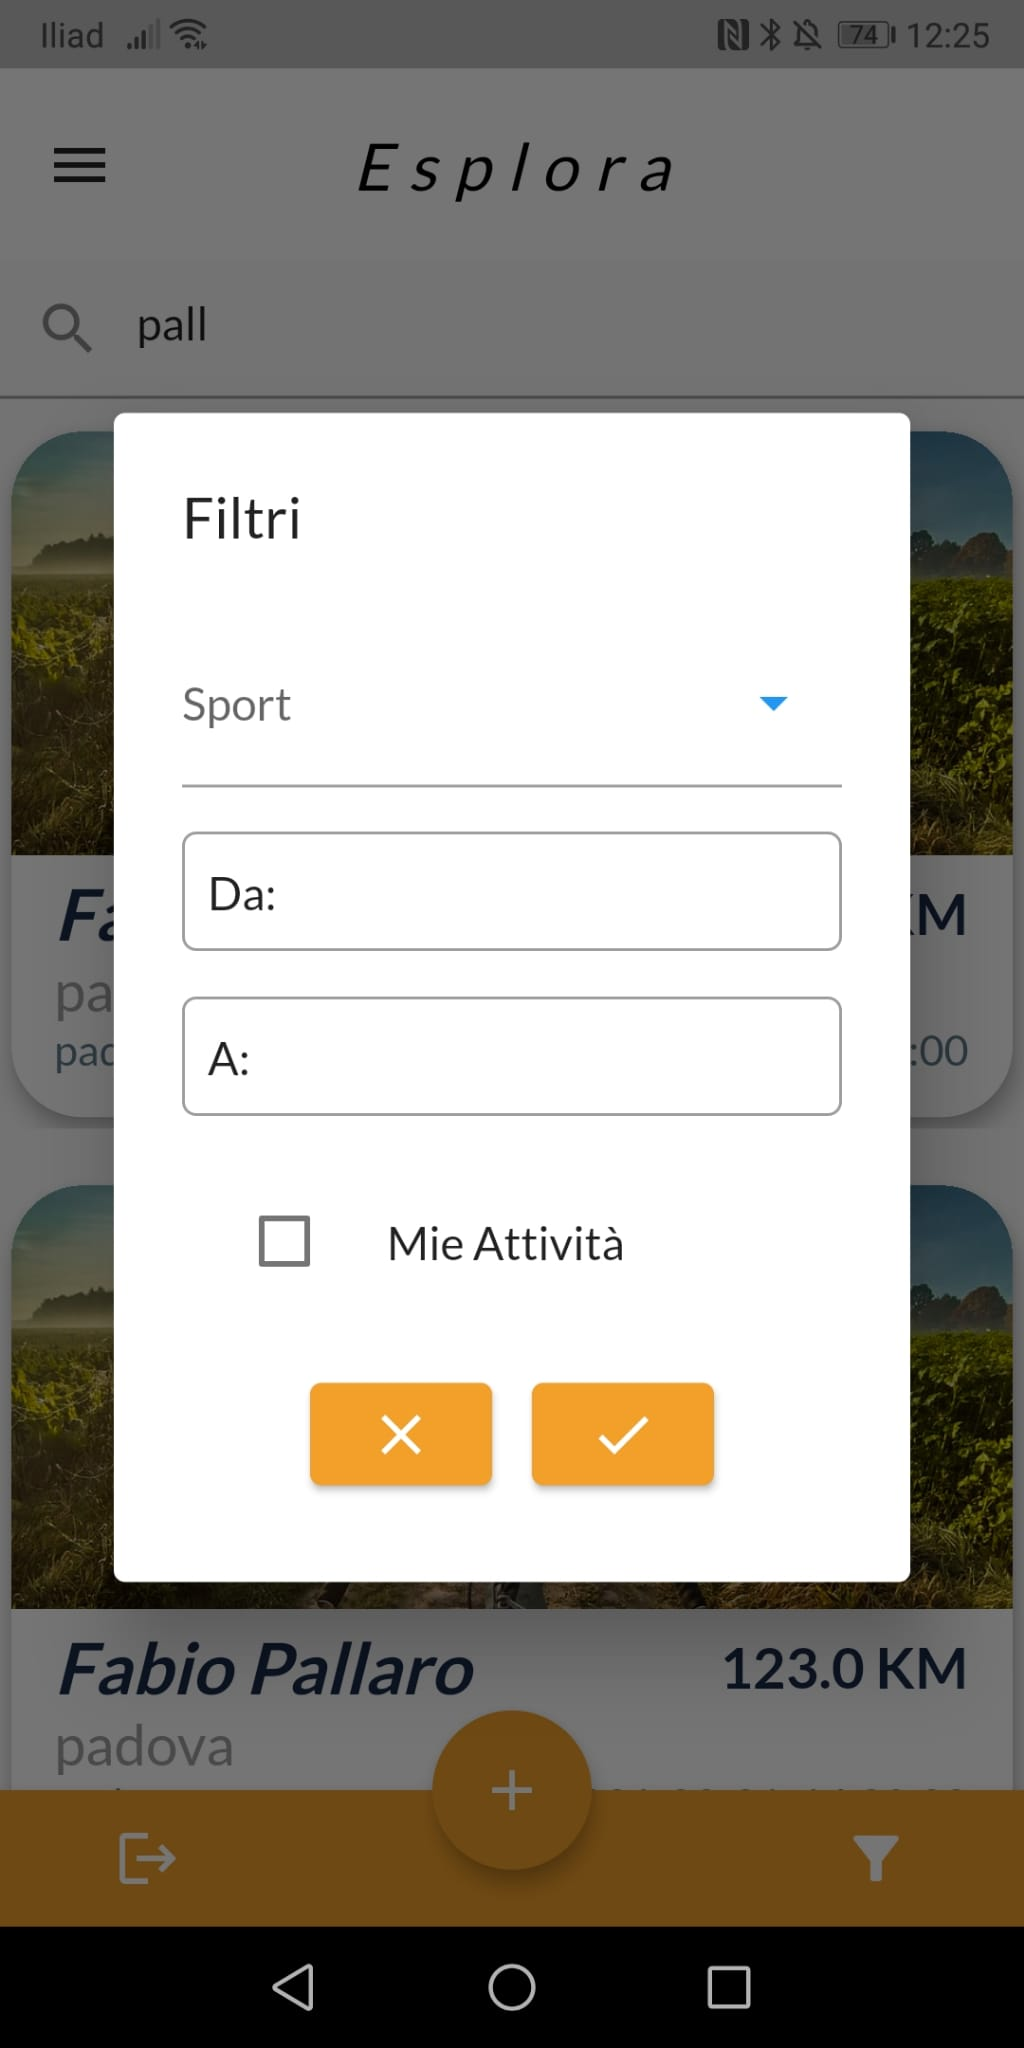
\includegraphics[width=6cm]{immagini/filtroavanzato.jpeg}
	\caption{Filtro avanzato di ricerca attività}
	\label{fig:Filtro avanzato di ricerca attività}
\end{figure}

\newpage

\subsection{Pubblicazione applicazione Play Store}
Questa è l'ultima attività effettuata che non è stata completata in modo pratico ma solo studiata anche se con molte probabilità in futuro è possibile che l'applicazione venga caricata sul Play Store.\\
Per pubblicare l'applicazione sul Play Store è stata studiata la documentazione fornita da Flutter al seguente indirizzo \url{https://flutter.dev/docs/deployment/android}.
Come prima cosa bisogna lanciare da terminale il seguente comando: \textit{keytool -genkey -v -keystore c:/Users/USER\_NAME/upload-keystore.jks -storetype JKS -keyalg RSA -keysize 2048 -validity 10000 -alias upload}, modificando il percorso.\\
Successivamente dopo aver fatto tutte le configurazioni necessarie bisognerà modificare il file key.properties con i valori appena configurati.\\
Dopo aver apportato le modifiche al file key.properties bisognerà modificare anche il file build.gradle come specificato dalla documentazione.\\
Infine bisognerà lanciare dal terminale prima il comando: \textit{flutter clean} e poi: \textit{flutter build appbundle}.\\
Infine per rilasciare l'applicazione bisognerà creare un account al seguente indirizzo \url{https://play.google.com/console/u/0/signup} pagando 25 dollari e successivamente, dopo aver superato tutti i test previsti, l'applicazione potrà essere rilasciata sul Play Store.\\

\begin{figure}[htbp]	
	\centering
	
\includegraphics[width=8cm]{immagini/playstore.jpg}
	\caption{Play Store}
	\label{fig:Play Store}
\end{figure}

